\chapter{Requirements Analysis}
\label{chap:requirements}

\section{Stakeholders and User Requirements}
\label{sec:stakeholders}

Three groups interact with the system, and their differing needs shape the requirements.

The \emph{anonymous visitor} arrives without an account. This group needs to browse public
videos, search and filter by category, and watch content immediately, because requiring
registration before any content can be seen would deter adoption. The \emph{registered user}
additionally needs to upload videos, control whether each video is public or private, manage
the videos on their own channel, and interact through likes and comments. The
\emph{system administrator}, in the context of this project the development team itself,
needs the platform to be observable and deployable without manual intervention.

\section{Functional Requirements}
\label{sec:functional-requirements}

Table~\ref{tab:functional-requirements} enumerates the functional requirements derived from the
stakeholder analysis. Each requirement is given an identifier so that it can be traced through
the design and implementation chapters.

\begin{table}[H]
\centering
\caption{Functional requirements of the system}
\label{tab:functional-requirements}
\small
\begin{tabularx}{\textwidth}{p{0.08\textwidth} p{0.22\textwidth} X}
\toprule
\textbf{ID} & \textbf{REQUIREMENT} & \textbf{DESCRIPTION} \\
\midrule
FR-01 & Registration and login & Users register with a username, email address, and password. Authentication uses JSON Web Tokens carried in the Authorization header. \\
FR-02 & Password recovery & Users request a reset link by email; the token is single-use and expires after fifteen minutes. \\
FR-03 & Direct upload to S3 & The client requests a pre-signed URL from the backend and transfers the file directly to Amazon S3 without routing the payload through the application server. \\
FR-04 & Automatic transcoding & Once the upload completes, the system transcodes the source into HLS renditions without any manual trigger. \\
FR-05 & Adaptive playback & The player switches automatically among 360p, 720p, and 1080p according to available bandwidth. \\
FR-06 & Visibility control & Each video is public or private, and the owner can change this setting after upload. \\
FR-07 & Channel management & Users view their own uploads, including those still processing, and may delete a video together with all of its stored artefacts. \\
FR-08 & Search and filtering & Users search by title, description, or tags, and filter by category. \\
FR-09 & Engagement & Users express likes and dislikes and post comments; a comment may be removed by its author or by the video owner. \\
FR-10 & View counting & The system records a view only after playback has genuinely started, and does not count repeated views from the same viewer within a short window. \\
\bottomrule
\end{tabularx}
\end{table}

Requirement FR-03 deserves particular comment because it shapes the architecture more than any
other functional requirement. Routing a multi-gigabyte upload through the backend would
consume server memory and bandwidth proportional to the number of concurrent uploads and would
make the API server the bottleneck of the entire platform. Issuing a time-limited pre-signed
URL and letting the browser transfer the file directly to Amazon S3 removes that bottleneck
entirely: the backend handles only a small JSON request regardless of file size.

\section{Non-Functional Requirements}
\label{sec:nonfunctional-requirements}

The non-functional requirements are stated in measurable terms wherever possible, so that
Chapter~\ref{chap:evaluation} can report whether they were met.

\begin{table}[H]
\centering
\caption{Non-functional requirements of the system}
\label{tab:nonfunctional-requirements}
\small
\begin{tabularx}{\textwidth}{p{0.08\textwidth} p{0.20\textwidth} X}
\toprule
\textbf{ID} & \textbf{ATTRIBUTE} & \textbf{REQUIREMENT} \\
\midrule
NFR-01 & Latency & Time-to-First-Frame should remain low enough that playback feels immediate; the measurement methodology is defined in Section~\ref{sec:qoe-evaluation}. \\
NFR-02 & Scalability & The pipeline must absorb a burst of concurrent uploads without losing work, processing them as capacity permits rather than rejecting them. \\
NFR-03 & Reliability & A failed transcoding job must not silently disappear: it must be retried where retrying could succeed, and must raise an alert carrying the reason when it cannot. The retry and alerting mechanisms that satisfy this requirement on the deployed path are described in Section~\ref{sec:challenges}. \\
NFR-04 & Cost efficiency & Compute cost must accrue only during actual transcoding, with no charge for idle capacity. \\
NFR-05 & Security of content & Private videos must be inaccessible to unauthorised viewers even when the exact manifest URL is known. \\
NFR-06 & Security of the API & Authentication endpoints must resist brute-force attempts, and the origin of cross-origin requests must be restricted to an explicit allow-list. \\
NFR-07 & Reproducibility & The entire infrastructure must be reproducible from source control through a single command. \\
NFR-08 & Maintainability & Changes must pass automated tests and security scanning before reaching the main branch. \\
\bottomrule
\end{tabularx}
\end{table}

Requirement NFR-05 is worth distinguishing from ordinary access control. Restricting an API
response is straightforward, but a video is not delivered by the API: it is delivered by a
content delivery network as hundreds of individual segment files. An access control scheme that
protects only the API therefore leaves the actual content unprotected, a gap that
Section~\ref{sec:content-protection} addresses explicitly.

\section{Use Case Model}
\label{sec:use-cases}

Figure~\ref{fig:use-case} presents the use case diagram of the system. Three actors appear: the
anonymous visitor, the authenticated user, and the transcoding system itself, which is modelled
as an actor because it initiates processing autonomously in response to events rather than in
response to a direct user action.

\begin{figure}[htbp]
\centering
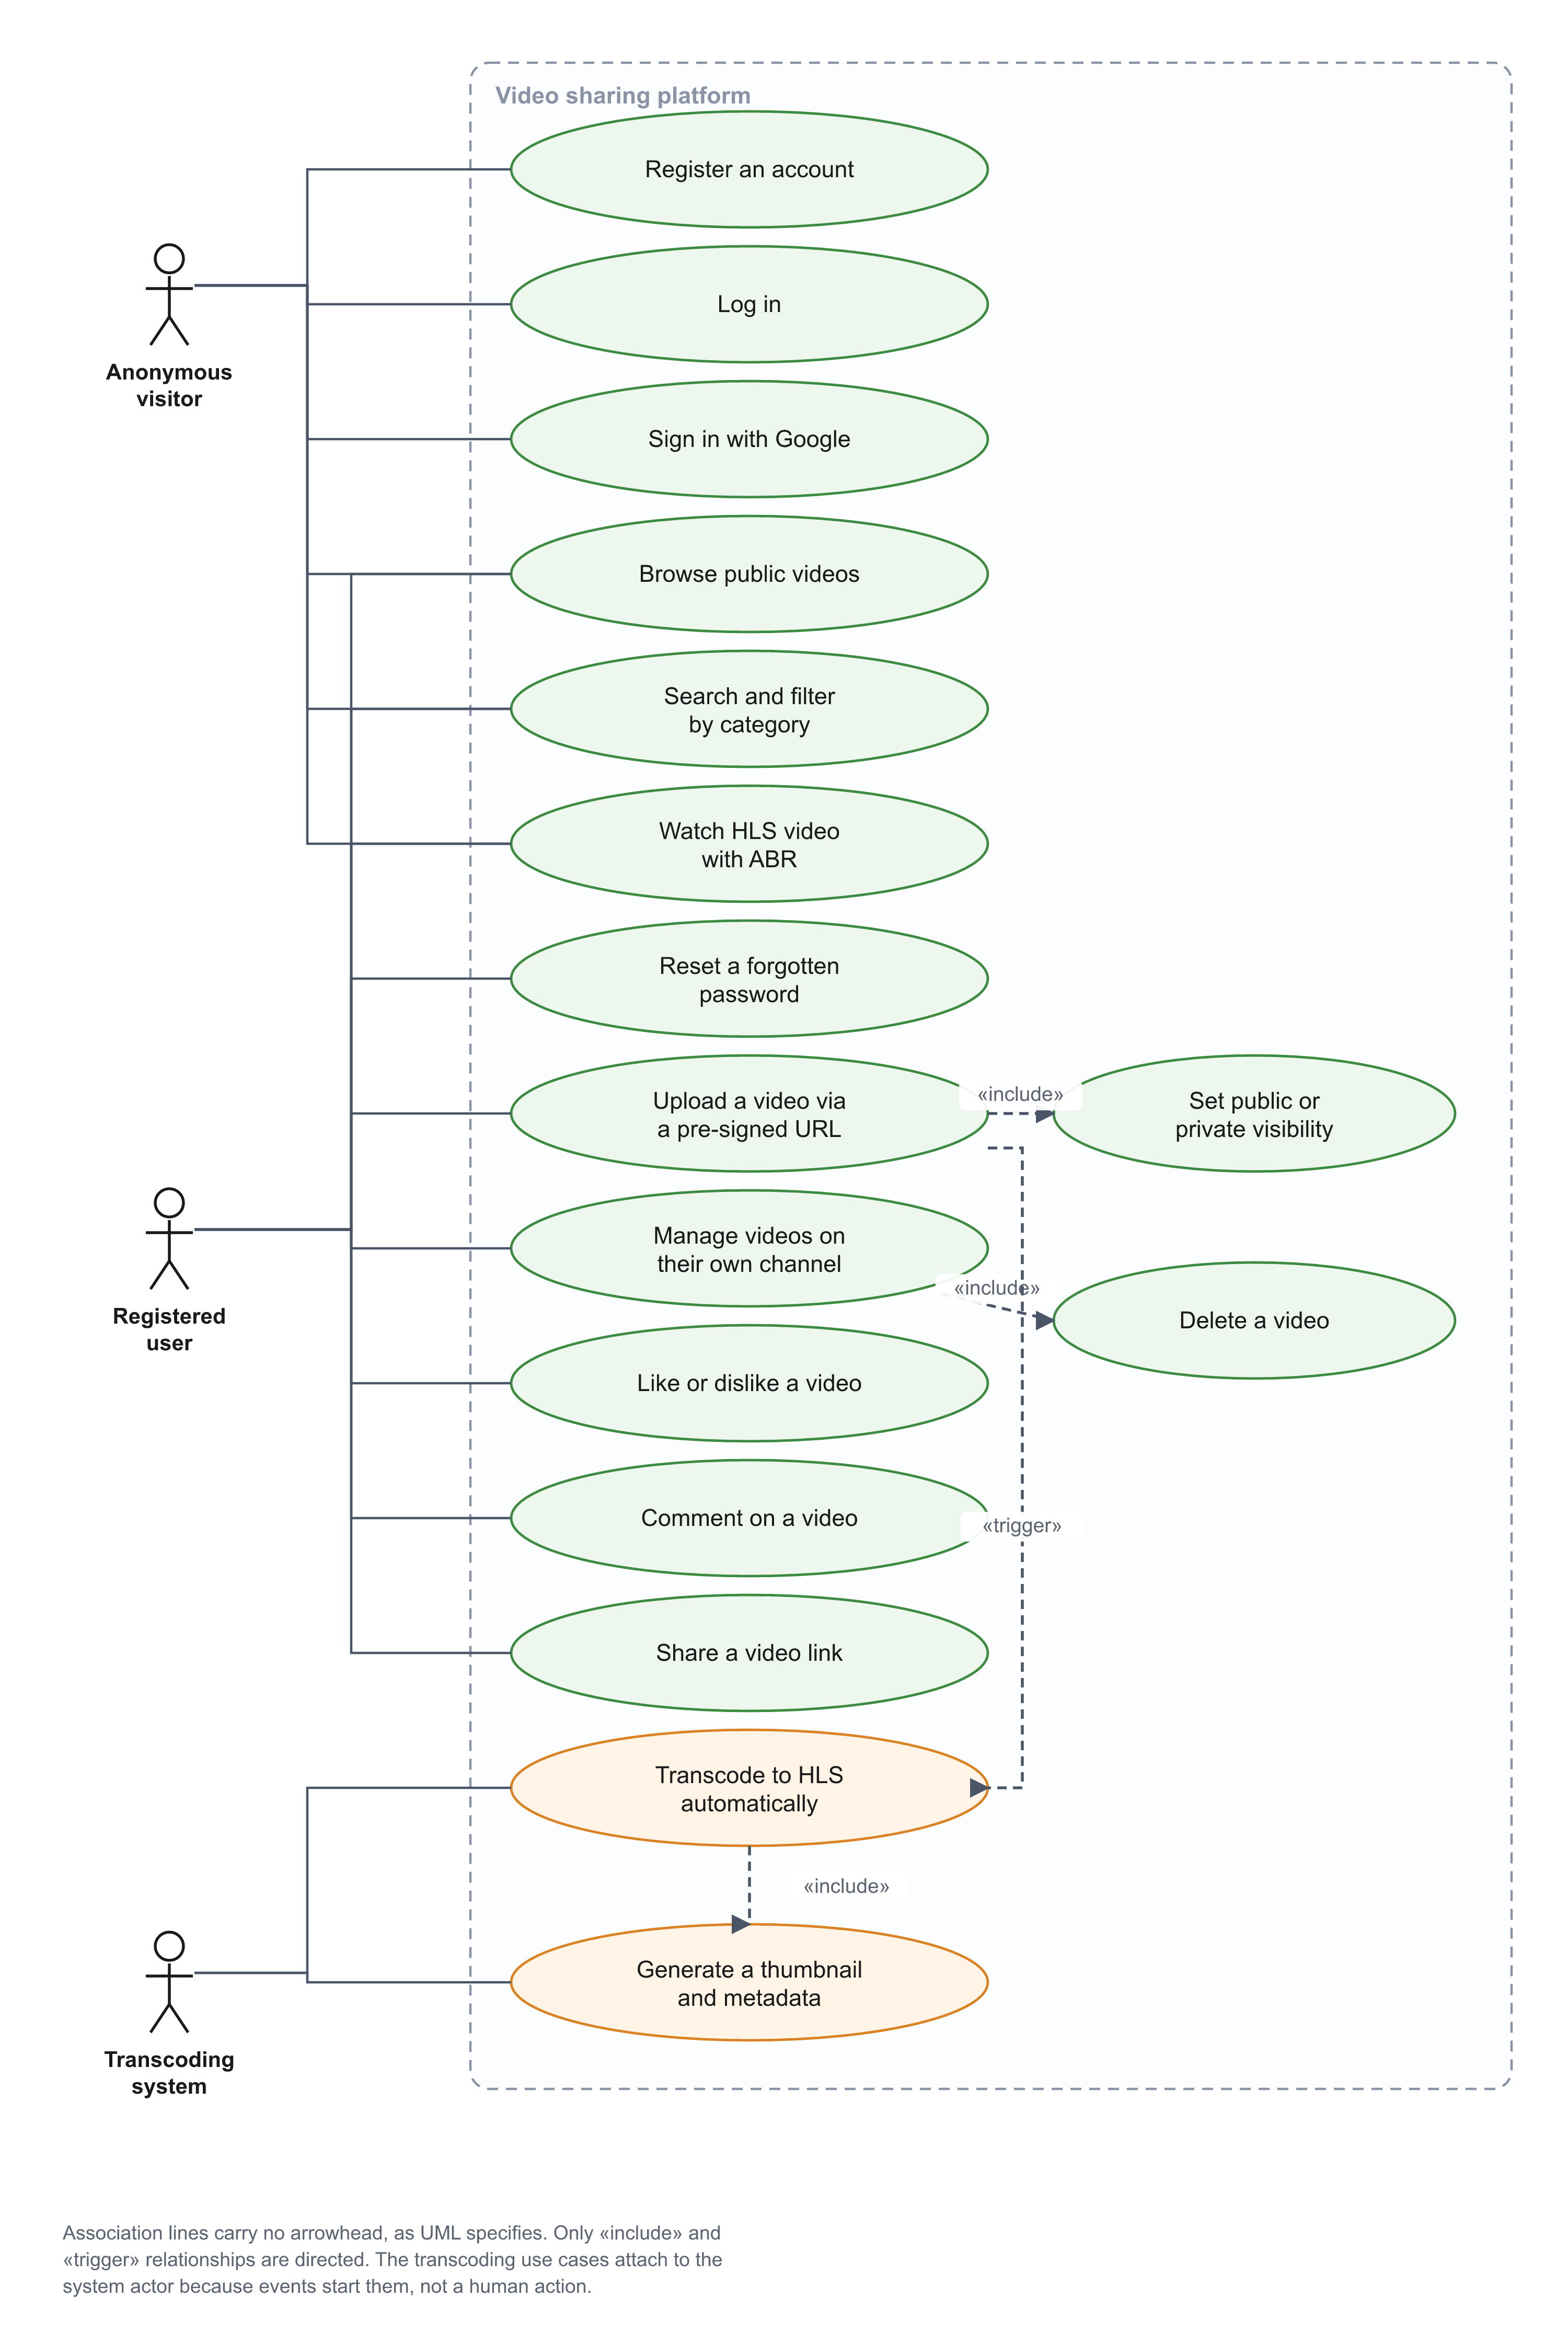
\includegraphics[width=0.92\textwidth]{images/05-use-case.png}
\caption{\textit{Use case diagram of the video sharing platform}}
\label{fig:use-case}
\end{figure}

The diagram makes visible an important property of the design: the transcoding use cases are
not invoked by the user at all. The user's upload action triggers them indirectly through the
event chain, which is why they are attached to the system actor rather than to the human
actors. This separation is what allows the browser to return control to the user immediately
after the upload completes, without waiting for processing to finish.

Table~\ref{tab:usecase-upload} specifies the most architecturally significant use case in
detail.

\begin{table}[H]
\centering
\caption{Use case specification: upload a video}
\label{tab:usecase-upload}
\small
\begin{tabularx}{\textwidth}{p{0.20\textwidth} X}
\toprule
\textbf{FIELD} & \textbf{CONTENT} \\
\midrule
Identifier & UC-07 \\
Actor & Authenticated user \\
Precondition & The user holds a valid JSON Web Token. \\
Trigger & The user selects a video file and submits the upload form. \\
Main flow &
  1. The client validates the file type and size locally. \newline
  2. The client calls the initiate-upload endpoint with the file metadata. \newline
  3. The server validates the metadata, creates a database record with status \texttt{UPLOADING}, and returns a pre-signed URL valid for fifteen minutes. \newline
  4. The browser transfers the file directly to the raw S3 bucket. \newline
  5. The client confirms completion and the record moves to \texttt{PROCESSING}. \newline
  6. The transcoding pipeline runs asynchronously and eventually sets the record to \texttt{READY}. \\
Alternative flow & If the file type is not an accepted video format or the size exceeds the limit, the server rejects the request before issuing a URL, and no orphan record is created. \\
Postcondition & The video appears on the user's channel, initially as processing and subsequently as ready to play. \\
\bottomrule
\end{tabularx}
\end{table}
